\section{eo\-PBILOrg$<$ EOT $>$ Class Template Reference}
\label{classeo_p_b_i_l_org}\index{eoPBILOrg@{eoPBILOrg}}
Distribution Class for PBIL algorithm (Population-Based Incremental Learning, Baluja and Caruana 95).  


{\tt \#include $<$eo\-PBILOrg.h$>$}

Inheritance diagram for eo\-PBILOrg$<$ EOT $>$::\begin{figure}[H]
\begin{center}
\leavevmode
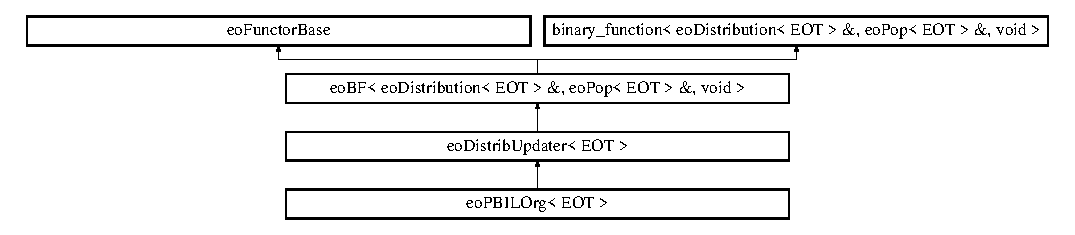
\includegraphics[height=2.71186cm]{classeo_p_b_i_l_org}
\end{center}
\end{figure}
\subsection*{Public Member Functions}
\begin{CompactItemize}
\item 
{\bf eo\-PBILOrg} (double \_\-LR, double \_\-tolerance=0.0)\label{classeo_p_b_i_l_org_a0}

\begin{CompactList}\small\item\em Ctor with size of genomes, and update parameters. \item\end{CompactList}\item 
virtual void {\bf operator()} ({\bf eo\-Distribution}$<$ {\bf EOT} $>$ \&\_\-distrib, {\bf eo\-Pop}$<$ {\bf EOT} $>$ \&\_\-pop)\label{classeo_p_b_i_l_org_a1}

\begin{CompactList}\small\item\em Update the distribution from the current population. \item\end{CompactList}\end{CompactItemize}
\subsection*{Private Attributes}
\begin{CompactItemize}
\item 
double {\bf LR}\label{classeo_p_b_i_l_org_r0}

\item 
double {\bf max\-Bound}\label{classeo_p_b_i_l_org_r1}

\item 
double {\bf min\-Bound}\label{classeo_p_b_i_l_org_r2}

\end{CompactItemize}


\subsection{Detailed Description}
\subsubsection*{template$<$class EOT$>$ class eo\-PBILOrg$<$ EOT $>$}

Distribution Class for PBIL algorithm (Population-Based Incremental Learning, Baluja and Caruana 95). 

This class implements the update rule from the original paper:

p(i)(t+1) = (1-LR)$\ast$p(i)(t) + LR$\ast$best(i) 



Definition at line 42 of file eo\-PBILOrg.h.

The documentation for this class was generated from the following file:\begin{CompactItemize}
\item 
eo\-PBILOrg.h\end{CompactItemize}
